\newpage
\section{模型的建立与求解}

\subsection{问题一的模型的建立和求解}

\subsubsection{模型建立}

预热平衡阶段，药材处于非稳态热风干燥初期。将药材视为长圆柱，忽略端面效应，温度场 $T(r,t)$ 与水分浓度场 $C(r,t)$ 仅沿径向 $r$ 变化，其控制方程由\textbf{热传导方程}与\textbf{水分扩散方程}构成：

\begin{equation}
	\rho c_p \frac{\partial T}{\partial t} = \frac{1}{r}\frac{\partial}{\partial r}\left(r k \frac{\partial T}{\partial r}\right), \qquad 0<r<R,\ t>0,
	\label{eq:heat}
\end{equation}
\begin{equation}
	\frac{\partial C}{\partial t} = \frac{1}{r}\frac{\partial}{\partial r}\left(r D \frac{\partial C}{\partial r}\right), \qquad 0<r<R,\ t>0,
	\label{eq:mass}
\end{equation}

其中 $\rho$ 为密度，$c_p$ 为比热容，$k$ 为热传导系数，$D$ 为水分扩散系数，$R$ 为药材半径。初始条件为

\begin{equation}
	T(r,0)=T_0=28\ ^\circ\text{C}, \qquad C(r,0)=C_0=2.55\ \text{kg/kg}.
	\label{eq:ic}
\end{equation}

在圆柱中心 $r=0$ 处由轴对称性给出对称边界条件，在表面 $r=R$ 处由牛顿冷却定律与对流传质定律给出第三类边界条件：

\begin{equation}
	\left.\frac{\partial T}{\partial r}\right|_{r=0}=0,\qquad
	\left.\frac{\partial C}{\partial r}\right|_{r=0}=0,
	\label{eq:bc0}
\end{equation}
\begin{equation}
	-k\left.\frac{\partial T}{\partial r}\right|_{r=R}=h\,(T-T_{air}),\qquad
	-D\left.\frac{\partial C}{\partial r}\right|_{r=R}=h_m\,(C-C_{air}),
	\label{eq:bcR}
\end{equation}

式中 $T_{air}(t)$、$C_{air}(t)$ 分别为烘房空气温度与水分浓度（附件 1），$h$、$h_m$ 分别为对流换热系数与对流传质系数。问题一中物性为常数（附录 2）：$\rho=820$ kg/m$^3$，$c_p=2600$ J/(kg$\cdot$K)，$k=0.36$ W/(m$\cdot$K)，$h=25$ W/(m$^2\cdot$K)，$h_m=8\times10^{-7}$ m/s，水分扩散系数满足经验公式

\begin{equation}
	D = 7\times10^{-9}\, e^{-0.89/C}.
	\label{eq:D1}
\end{equation}

\subsubsection{数值方法}

方程组 \eqref{eq:heat}--\eqref{eq:mass} 为非线性耦合偏微分方程组（$D$ 依赖 $C$），本文采用\textbf{控制体积法}在空间离散、\textbf{Crank--Nicolson 隐式格式}在时间离散。取均匀网格 $r_i=i\Delta r$（$i=0,1,\dots,N$，$\Delta r=R/N$），对方程 \eqref{eq:heat} 在第 $i$ 个控制体积上积分，可得半离散形式

\begin{equation}
	\frac{d T_i}{dt} = \frac{2}{r_{i,R}^2-r_{i,L}^2}\left[\frac{r_{i,R}\, k_{i+1/2}}{\Delta r}(T_{i+1}-T_i)-\frac{r_{i,L}\, k_{i-1/2}}{\Delta r}(T_i-T_{i-1})\right],
	\label{eq:discheat}
\end{equation}

其中 $r_{i,L}=r_i-\Delta r/2$、$r_{i,R}=r_i+\Delta r/2$ 为控制体积左右界面，$k_{i\pm1/2}$ 为界面导热系数。中心节点由对称条件退化为 $\dfrac{dT_0}{dt}=\dfrac{4k_{1/2}}{\rho c_p\Delta r^2}(T_1-T_0)$；表面节点用边界条件 \eqref{eq:bcR} 处理。水分方程 \eqref{eq:mass} 的离散完全类似（以 $D$ 代 $k$，去掉 $\rho c_p$，以 $h_m$ 代 $h$）。记离散后系统为 $du/dt=Lu+b$，Crank--Nicolson 格式为

\begin{equation}
	\left(I-\frac{\Delta t}{2}L\right) u^{n+1} = \left(I+\frac{\Delta t}{2}L\right) u^{n} + \frac{\Delta t}{2}\left(b^{n+1}+b^n\right),
	\label{eq:cn}
\end{equation}

每步求解三对角线性方程组（用 Thomas 追赶法/\texttt{scipy.linalg.solve\_banded}）\cite{crank1947practical}。传热与传质之间的耦合（$D$ 依赖 $C$、$T$）通过每个时间步内的固定点迭代处理，迭代至收敛。相关传热与数值传热理论参见文献 \cite{yang2006heat,tao2001numerical}。求解采用 $\Delta r=0.005$ cm（$N=400$）、$\Delta t=0.5$ s，经收敛性检验（见第 \ref{sec:check} 节）满足四位小数精度要求。

\subsubsection{模型求解}

利用附件 1 的烘房温湿度作为边界输入，求解得到预热平衡阶段药材温度与水分浓度分布，结果如表~\ref{tab:p1-temperature}、表~\ref{tab:p1-moisture} 所示（完整结果见 result1.xlsx）。

\begin{table}[htbp]
	\caption{30 分钟内药材的温度（°C）}
	\label{tab:p1-temperature}
	\centering
	\begin{tabular}{cccccc}
		\toprule
		\multirow{2}{*}{时间/s} & \multicolumn{5}{c}{到药材中心的距离/cm} \\
		\cmidrule(lr){2-6}
		 & 0 & 0.5 & 1 & 1.5 & 2 \\
		\midrule
		100 & 28.0001 & 28.0003 & 28.0040 & 28.0327 & 28.1801 \\
		300 & 28.0408 & 28.0635 & 28.1514 & 28.3681 & 28.8488 \\
		600 & 28.4533 & 28.5360 & 28.8039 & 29.3159 & 30.1652 \\
		900 & 29.3243 & 29.4583 & 29.8755 & 30.6161 & 31.7304 \\
		1200 & 30.5427 & 30.7098 & 31.2223 & 32.1126 & 33.4276 \\
		1500 & 31.9957 & 32.1867 & 32.7660 & 33.7463 & 35.1203 \\
		1800 & 33.5753 & 33.7720 & 34.3642 & 35.3621 & 36.7856 \\
		\bottomrule
	\end{tabular}
\end{table}

\begin{table}[htbp]
	\caption{30 分钟内药材的水分浓度（kg/kg）}
	\label{tab:p1-moisture}
	\centering
	\begin{tabular}{cccccc}
		\toprule
		\multirow{2}{*}{时间/s} & \multicolumn{5}{c}{到药材中心的距离/cm} \\
		\cmidrule(lr){2-6}
		 & 0 & 0.5 & 1 & 1.5 & 2 \\
		\midrule
		100 & 2.5500 & 2.5500 & 2.5500 & 2.5500 & 2.2471 \\
		300 & 2.5500 & 2.5500 & 2.5500 & 2.5492 & 2.0509 \\
		600 & 2.5500 & 2.5500 & 2.5500 & 2.5353 & 1.8770 \\
		900 & 2.5500 & 2.5500 & 2.5497 & 2.5045 & 1.7547 \\
		1200 & 2.5500 & 2.5500 & 2.5482 & 2.4646 & 1.6586 \\
		1500 & 2.5500 & 2.5499 & 2.5445 & 2.4206 & 1.5787 \\
		1800 & 2.5500 & 2.5497 & 2.5383 & 2.3755 & 1.5102 \\
		\bottomrule
	\end{tabular}
\end{table}

\begin{figure}[htbp]
	\centering
	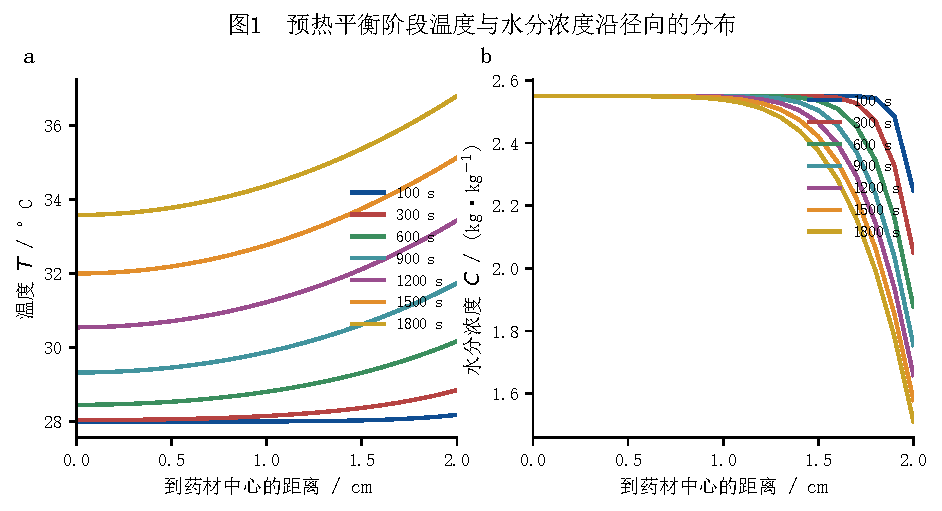
\includegraphics[width=0.98\textwidth]{texfile/figures/fig1_p1_profiles.pdf}
	\caption{预热平衡阶段温度（a）与水分浓度（b）沿径向的分布}
	\label{fig:p1-profiles}
\end{figure}

\begin{figure}[htbp]
	\centering
	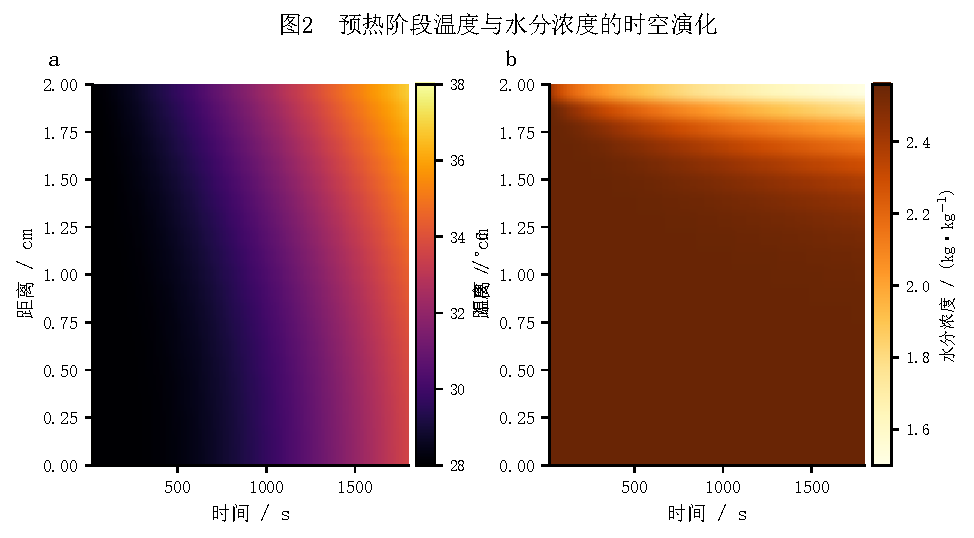
\includegraphics[width=0.98\textwidth]{texfile/figures/fig2_p1_spacetime.pdf}
	\caption{预热平衡阶段温度（a）与水分浓度（b）的时空演化}
	\label{fig:p1-spacetime}
\end{figure}

由图~\ref{fig:p1-profiles}、图~\ref{fig:p1-spacetime} 可见：预热阶段热量由表面向中心\textbf{由外向内逐步渗透}，$1800$ s 时表面温度 $36.79$ °C 明显高于中心 $33.58$ °C，且尚未追平烘房温度（$1800$ s 时约 $41.5$ °C），说明预热尚未完成；而水分仅在表面附近有可察觉的下降（$1800$ s 时表面降至 $1.510$ kg/kg），中心区域基本维持初始值 $2.55$ kg/kg。这是因为水分的扩散系数极小（约 $5\times10^{-9}$ m$^2$/s），扩散时间尺度远大于温度的热扩散时间尺度，故 30 min 内水分输运仅局限于表层。

\subsection{问题二的模型的建立和求解}

\subsubsection{变物性模型}

问题二要求建立整个烘干过程的模型。此时药材含水率在很大范围内变化，物性不再为常数，采用附录 3 的经验公式：

\begin{equation}
	\rho = 650+128C, \qquad
	c_p = 1450+2736\frac{C}{C+1}, \qquad
	k = 0.21+0.38\frac{C}{C+1},
	\label{eq:props3}
\end{equation}
\begin{equation}
	D = 2.4\times10^{-3}\, e^{-0.45/C}\, e^{-3850/T},
	\label{eq:D3}
\end{equation}

其中 $T$ 为热力学温度（K）。方程 \eqref{eq:heat}--\eqref{eq:mass} 及其边界条件保持不变，仅物性由 \eqref{eq:props3}、\eqref{eq:D3} 给定。烘房环境分两段：预热段（$0\sim4$ h）采用附件 1 实测温湿度线性插值，恒温段（$4$ h 之后）取 $T_{air}=50$ °C、$C_{air}=0.050$ kg/kg。求解方法与问题一相同，网格 $\Delta r=0.005$ cm、$\Delta t=1$ s。

\subsubsection{模型求解}

表~\ref{tab:p2-temperature}、表~\ref{tab:p2-moisture} 给出 3 h 内每隔 0.5 h 的温度与水分浓度（完整结果见 result2.xlsx），图~\ref{fig:p2-profiles}、图~\ref{fig:p2-timeseries} 展示其时空演化。

\begin{table}[htbp]
	\caption{3 小时内药材的温度（°C）}
	\label{tab:p2-temperature}
	\centering
	\begin{tabular}{cccccc}
		\toprule
		\multirow{2}{*}{时间/h} & \multicolumn{5}{c}{到药材中心的距离/cm} \\
		\cmidrule(lr){2-6}
		 & 0 & 0.5 & 1 & 1.5 & 2 \\
		\midrule
		0.5 & 32.1892 & 32.3821 & 32.9659 & 33.9608 & 35.4130 \\
		1.0 & 40.3816 & 40.5536 & 41.0605 & 41.8782 & 42.9976 \\
		1.5 & 45.8468 & 45.9348 & 46.1930 & 46.6051 & 47.1401 \\
		2.0 & 48.4502 & 48.4881 & 48.5984 & 48.7736 & 49.0033 \\
		2.5 & 49.4670 & 49.4792 & 49.5137 & 49.5653 & 49.6609 \\
		3.0 & 49.8495 & 49.8553 & 49.8746 & 49.9101 & 49.9664 \\
		\bottomrule
	\end{tabular}
\end{table}

\begin{table}[htbp]
	\caption{3 小时内药材的水分浓度（kg/kg）}
	\label{tab:p2-moisture}
	\centering
	\begin{tabular}{cccccc}
		\toprule
		\multirow{2}{*}{时间/h} & \multicolumn{5}{c}{到药材中心的距离/cm} \\
		\cmidrule(lr){2-6}
		 & 0 & 0.5 & 1 & 1.5 & 2 \\
		\midrule
		0.5 & 2.5499 & 2.5489 & 2.5256 & 2.3257 & 1.6486 \\
		1.0 & 2.5257 & 2.4948 & 2.3578 & 2.0230 & 1.4711 \\
		1.5 & 2.3861 & 2.3256 & 2.1344 & 1.8020 & 1.3476 \\
		2.0 & 2.1709 & 2.1084 & 1.9236 & 1.6259 & 1.2311 \\
		2.5 & 1.9566 & 1.9006 & 1.7360 & 1.4720 & 1.1166 \\
		3.0 & 1.7662 & 1.7165 & 1.5702 & 1.3333 & 1.0081 \\
		\bottomrule
	\end{tabular}
\end{table}

\begin{figure}[htbp]
	\centering
	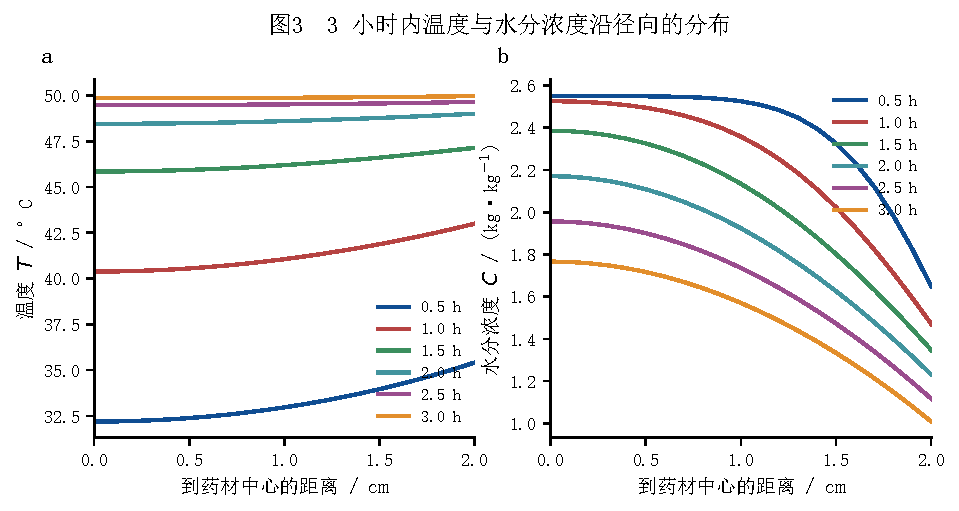
\includegraphics[width=0.98\textwidth]{texfile/figures/fig3_p2_profiles.pdf}
	\caption{3 小时内温度（a）与水分浓度（b）沿径向的分布}
	\label{fig:p2-profiles}
\end{figure}

\begin{figure}[htbp]
	\centering
	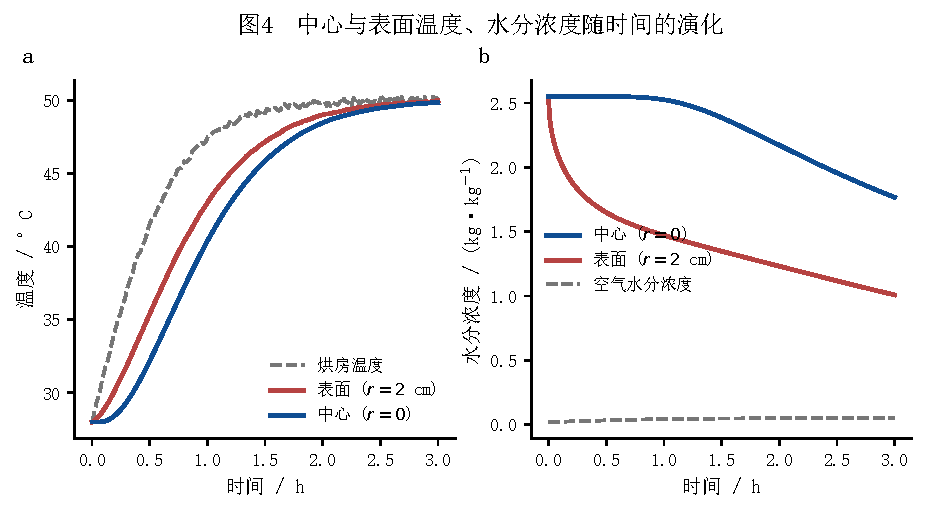
\includegraphics[width=0.98\textwidth]{texfile/figures/fig4_p2_timeseries.pdf}
	\caption{中心与表面温度（a）、水分浓度（b）随时间的演化}
	\label{fig:p2-timeseries}
\end{figure}

\begin{figure}[htbp]
	\centering
	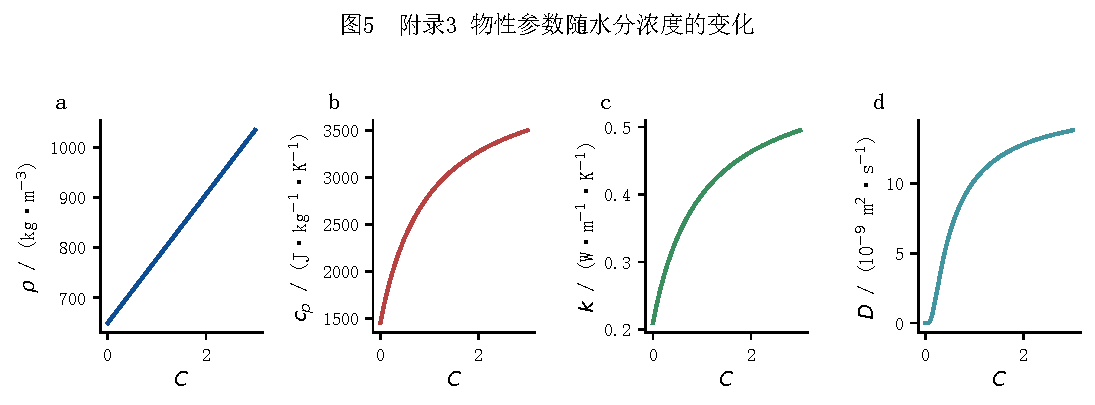
\includegraphics[width=0.98\textwidth]{texfile/figures/fig5_p2_properties.pdf}
	\caption{附录 3 物性参数 $\rho$、$c_p$、$k$、$D$ 随水分浓度 $C$ 的变化}
	\label{fig:p2-properties}
\end{figure}

由图~\ref{fig:p2-timeseries} 可见，药材温度约在 $1.5\sim2$ h 内完成预热并趋于均匀，$3$ h 时各处温度已逼近烘房温度 $50$ °C（$49.85\sim49.97$ °C）；水分则由表及里持续下降，且表面下降快、中心下降慢，径向梯度随时间逐渐形成并发展。图~\ref{fig:p2-properties} 表明，密度、比热容、导热系数随含水率近似线性或饱和式增大，而扩散系数 $D$ 同时受含水率与温度的强烈控制，随含水率下降、温度升高呈数量级变化，这决定了变物性建模的必要性。

\subsection{问题三的模型的建立和求解}

\subsubsection{求解思路}

问题三沿用问题二的变物性模型（附录 3），目标是确定满足“药材各处水分浓度均低于 $0.15$ kg/kg”的\textbf{最短干燥时间}。由于中心处距离表面最远、水分最难逸出，全场最大含水率始终出现在中心 $r=0$ 处，故烘干判据等价于

\begin{equation}
	\max_{0\le r\le R} C(r,t) = C(0,t) < 0.15\ \text{kg/kg}.
	\label{eq:judge}
\end{equation}

将模型从 $t=0$ 积分，在每一步检查判据 \eqref{eq:judge}，首次满足的时刻即为烘干结束时间 $t^*$。求解采用 $\Delta r=0.005$ cm、$\Delta t=5$ s，输出每 60 s 的水分浓度场（完整结果见 result3.xlsx）。

\subsubsection{模型求解}

计算得到\textbf{烘干结束时间 $t^*=206825$ s $=57.45$ h（约 2.39 天）}，与题目给出的“2--3 天”量级一致。表~\ref{tab:p3-moisture} 给出每隔 6 h 及结束时刻的水分浓度分布。

\begin{table}[htbp]
	\caption{药材烘干过程的水分浓度（kg/kg）}
	\label{tab:p3-moisture}
	\centering
	\begin{tabular}{cccccc}
		\toprule
		\multirow{2}{*}{时间/h} & \multicolumn{5}{c}{到药材中心的距离/cm} \\
		\cmidrule(lr){2-6}
		 & 0 & 0.5 & 1 & 1.5 & 2 \\
		\midrule
		6 & 1.0170 & 0.9881 & 0.9015 & 0.7550 & 0.5328 \\
		12 & 0.4561 & 0.4432 & 0.4031 & 0.3297 & 0.1642 \\
		18 & 0.2988 & 0.2915 & 0.2687 & 0.2253 & 0.0845 \\
		24 & 0.2378 & 0.2327 & 0.2167 & 0.1855 & 0.0665 \\
		30 & 0.2058 & 0.2018 & 0.1891 & 0.1641 & 0.0598 \\
		36 & 0.1859 & 0.1825 & 0.1718 & 0.1503 & 0.0566 \\
		42 & 0.1720 & 0.1691 & 0.1597 & 0.1407 & 0.0549 \\
		48 & 0.1618 & 0.1592 & 0.1507 & 0.1334 & 0.0537 \\
		54 & 0.1538 & 0.1514 & 0.1436 & 0.1277 & 0.0530 \\
		57.45 & 0.1500 & 0.1477 & 0.1402 & 0.1249 & 0.0527 \\
		\bottomrule
	\end{tabular}
\end{table}

\begin{figure}[htbp]
	\centering
	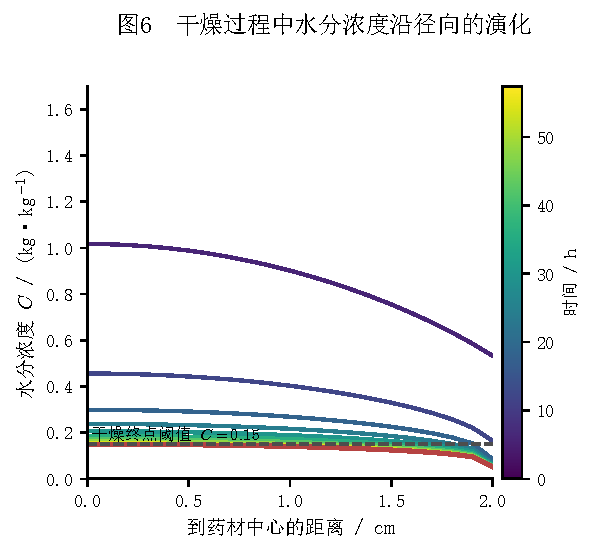
\includegraphics[width=0.52\textwidth]{texfile/figures/fig6_p3_profiles.pdf}
	\caption{干燥过程中水分浓度沿径向的演化}
	\label{fig:p3-profiles}
\end{figure}

\begin{figure}[htbp]
	\centering
	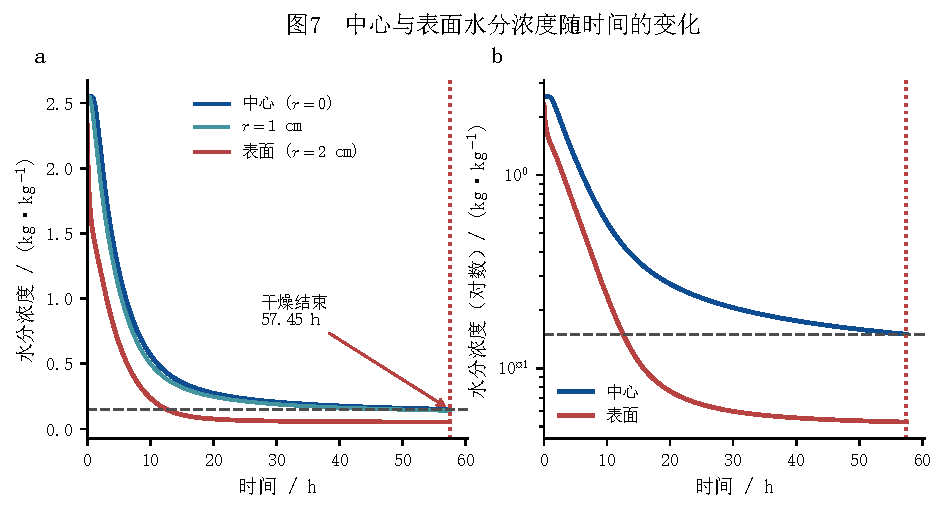
\includegraphics[width=0.98\textwidth]{texfile/figures/fig7_p3_drying.pdf}
	\caption{中心与表面水分浓度随时间的变化（a：线性坐标；b：对数坐标）}
	\label{fig:p3-drying}
\end{figure}

\begin{figure}[htbp]
	\centering
	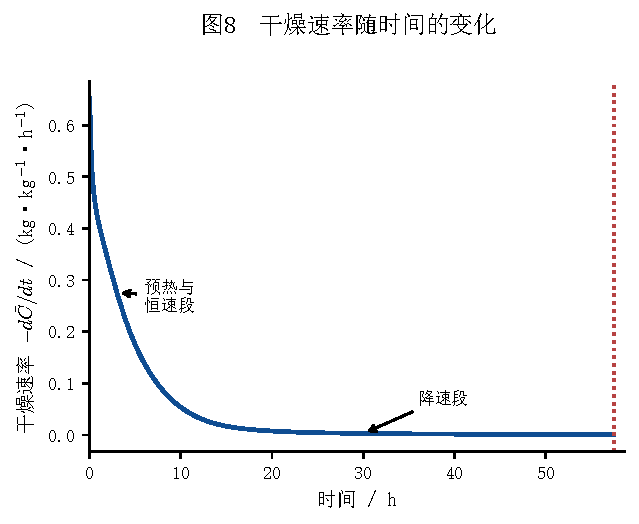
\includegraphics[width=0.55\textwidth]{texfile/figures/fig8_p3_rate.pdf}
	\caption{干燥速率随时间的变化}
	\label{fig:p3-rate}
\end{figure}

\begin{figure}[htbp]
	\centering
	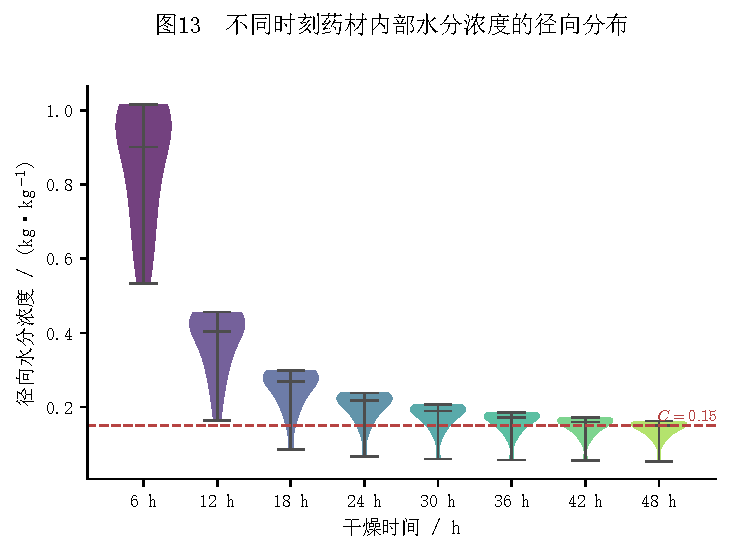
\includegraphics[width=0.72\textwidth]{texfile/figures/fig13_violin.pdf}
	\caption{不同时刻药材内部水分浓度的径向分布（小提琴图）}
	\label{fig:p3-violin}
\end{figure}

由图~\ref{fig:p3-profiles}、图~\ref{fig:p3-drying} 可见：表面含水率在数小时内迅速下降并趋近空气平衡值（$\approx0.05$ kg/kg），中心含水率下降缓慢，是制约干燥周期的“瓶颈”；干燥过程呈现明显的\textbf{恒速段与降速段}（图~\ref{fig:p3-rate}），前期表面水分充足、干燥速率较高，后期受内部扩散控制、速率持续衰减，直至 $57.45$ h 时全场含水率降至 $0.15$ kg/kg 以下。图~\ref{fig:p3-violin} 以小提琴图刻画了各时刻径向水分浓度的分布形态：随干燥进行，分布整体下移且“琴体”逐渐收窄，表明径向水分梯度不断减小、内部水分趋于均匀。

\subsection{问题四的模型的建立和求解}

\subsubsection{移动边界模型}

实际烘干中，药材因失水发生尺寸收缩。附件 2 给出了半径 $R(t)$ 随时间的变化（$2\to1.198$ cm）。为抑制三次样条插值可能出现的非物理振荡，本文采用\textbf{保单调三次插值（PCHIP）}拟合 $R(t)$。在固定网格 $r_i=i\Delta r$（$\Delta r=R_0/N$，$R_0=2$ cm）上，每个时刻由 $R(t)$ 确定活动节点数 $M=\lfloor R(t)/\Delta r\rfloor$，表面边界落在最后一格内（宽度 $\delta=R(t)-M\Delta r$）。将表面薄层与对流传质阻力串联，可得等效传质系数

\begin{equation}
	h_{m,eff}=\frac{1}{1/h_m+\delta/D}, \qquad
	h_{eff}=\frac{1}{1/h+\delta/k},
	\label{eq:heff}
\end{equation}

从而在固定网格上实现\textbf{移动边界}处理；物性采用附录 4 经验公式

\begin{equation}
	\rho = 760+90C,\qquad c_p = 1850+2150\frac{C}{C+1},\qquad k = 0.12+0.20\frac{C}{C+1},
	\label{eq:props4}
\end{equation}
\begin{equation}
	D = 4.2\times10^{-4}\, e^{-0.30/C}\, e^{-3850/T}.
	\label{eq:D4}
\end{equation}

其余控制方程、边界条件与求解方法同前（$\Delta r=0.005$ cm、$\Delta t=5$ s），输出每 60 s 的水分浓度场（完整结果见 result4.xlsx）。

\subsubsection{模型求解}

计算得到\textbf{烘干结束时间 $t^*=189470$ s $=52.63$ h（约 2.19 天）}，结束时刻表面半径 $R=1.200$ cm。表~\ref{tab:p4-moisture} 给出每隔 6 h 及结束时刻的水分浓度分布（因半径收缩，表面距离小于 1.5 cm 后相应列以“—”表示）。

\begin{table}[htbp]
	\caption{药材烘干过程的水分浓度（kg/kg，考虑尺寸收缩）}
	\label{tab:p4-moisture}
	\centering
	\begin{tabular}{cccccc}
		\toprule
		\multirow{2}{*}{时间/h} & \multicolumn{5}{c}{到药材中心的距离/cm} \\
		\cmidrule(lr){2-6}
		 & 0 & 0.5 & 1 & 1.5 & 药材表面 \\
		\midrule
		6 & 1.9516 & 1.7822 & 1.2568 & — & 0.5668 \\
		12 & 0.8733 & 0.7763 & 0.4858 & — & 0.2144 \\
		18 & 0.4593 & 0.4130 & 0.2651 & — & 0.1021 \\
		24 & 0.3071 & 0.2805 & 0.1901 & — & 0.0714 \\
		30 & 0.2380 & 0.2197 & 0.1553 & — & 0.0610 \\
		36 & 0.1999 & 0.1860 & 0.1355 & — & 0.0567 \\
		42 & 0.1760 & 0.1647 & 0.1226 & — & 0.0545 \\
		48 & 0.1596 & 0.1499 & 0.1135 & — & 0.0532 \\
		52.63 & 0.1500 & 0.1413 & 0.1081 & — & 0.0526 \\
		\bottomrule
	\end{tabular}
\end{table}

\begin{figure}[htbp]
	\centering
	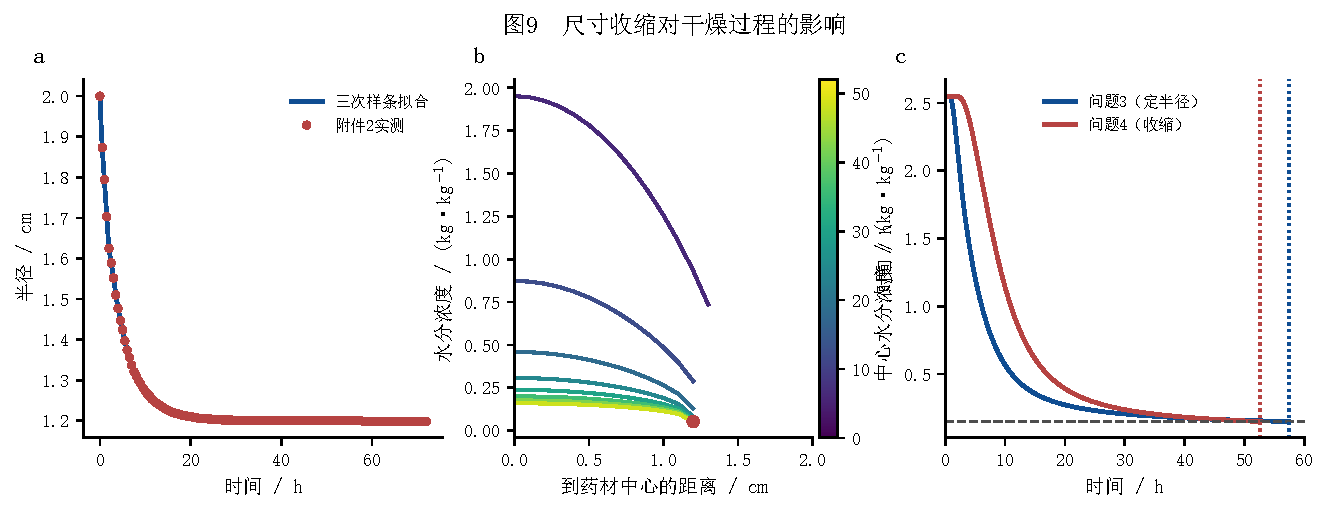
\includegraphics[width=0.98\textwidth]{texfile/figures/fig9_p4_shrinkage.pdf}
	\caption{尺寸收缩对干燥过程的影响（a：半径变化；b：收缩域水分剖面；c：问题 3/4 中心含水率对比）}
	\label{fig:p4-shrinkage}
\end{figure}

由图~\ref{fig:p4-shrinkage} 可见：半径由 $2$ cm 单调收缩至约 $1.2$ cm，收缩使有效扩散路径缩短，从而在后半程加快干燥；但因附录 4 的扩散系数整体小于附录 3，问题四前期干燥较慢，最终在 $52.63$ h 完成，较问题三的 $57.45$ h 略短。二者结果相互印证，说明移动边界模型能够合理刻画失水收缩对干燥进程的影响。
